\section{Fraktální dimenze}\label{sec:fraktalni_dimenze}

\subsection{Chápání konceptu dimenze}\label{subsec:koncept-dimenze}

Výčet útvarů v sekci \ref{sec:sobepodobnost} splňoval zásadní vlastnost, a to sice, že všechny z nich byly \emph{soběpodobné}. V eukleidovské geometrii lze však u mnohých základních objektů pozorovat stejnou vlastnost. Např. čtverec lze určitě prohlásit v jistém smyslu za soběpodobný, neboť jej lze rozdělit na podobné útvary (viz obrázek \ref{fig:sobepodobnost-ctverce}).
\begin{figure}[h]
    \centering
    \begin{subfigure}[b]{\subfigwidth}
        \centering
        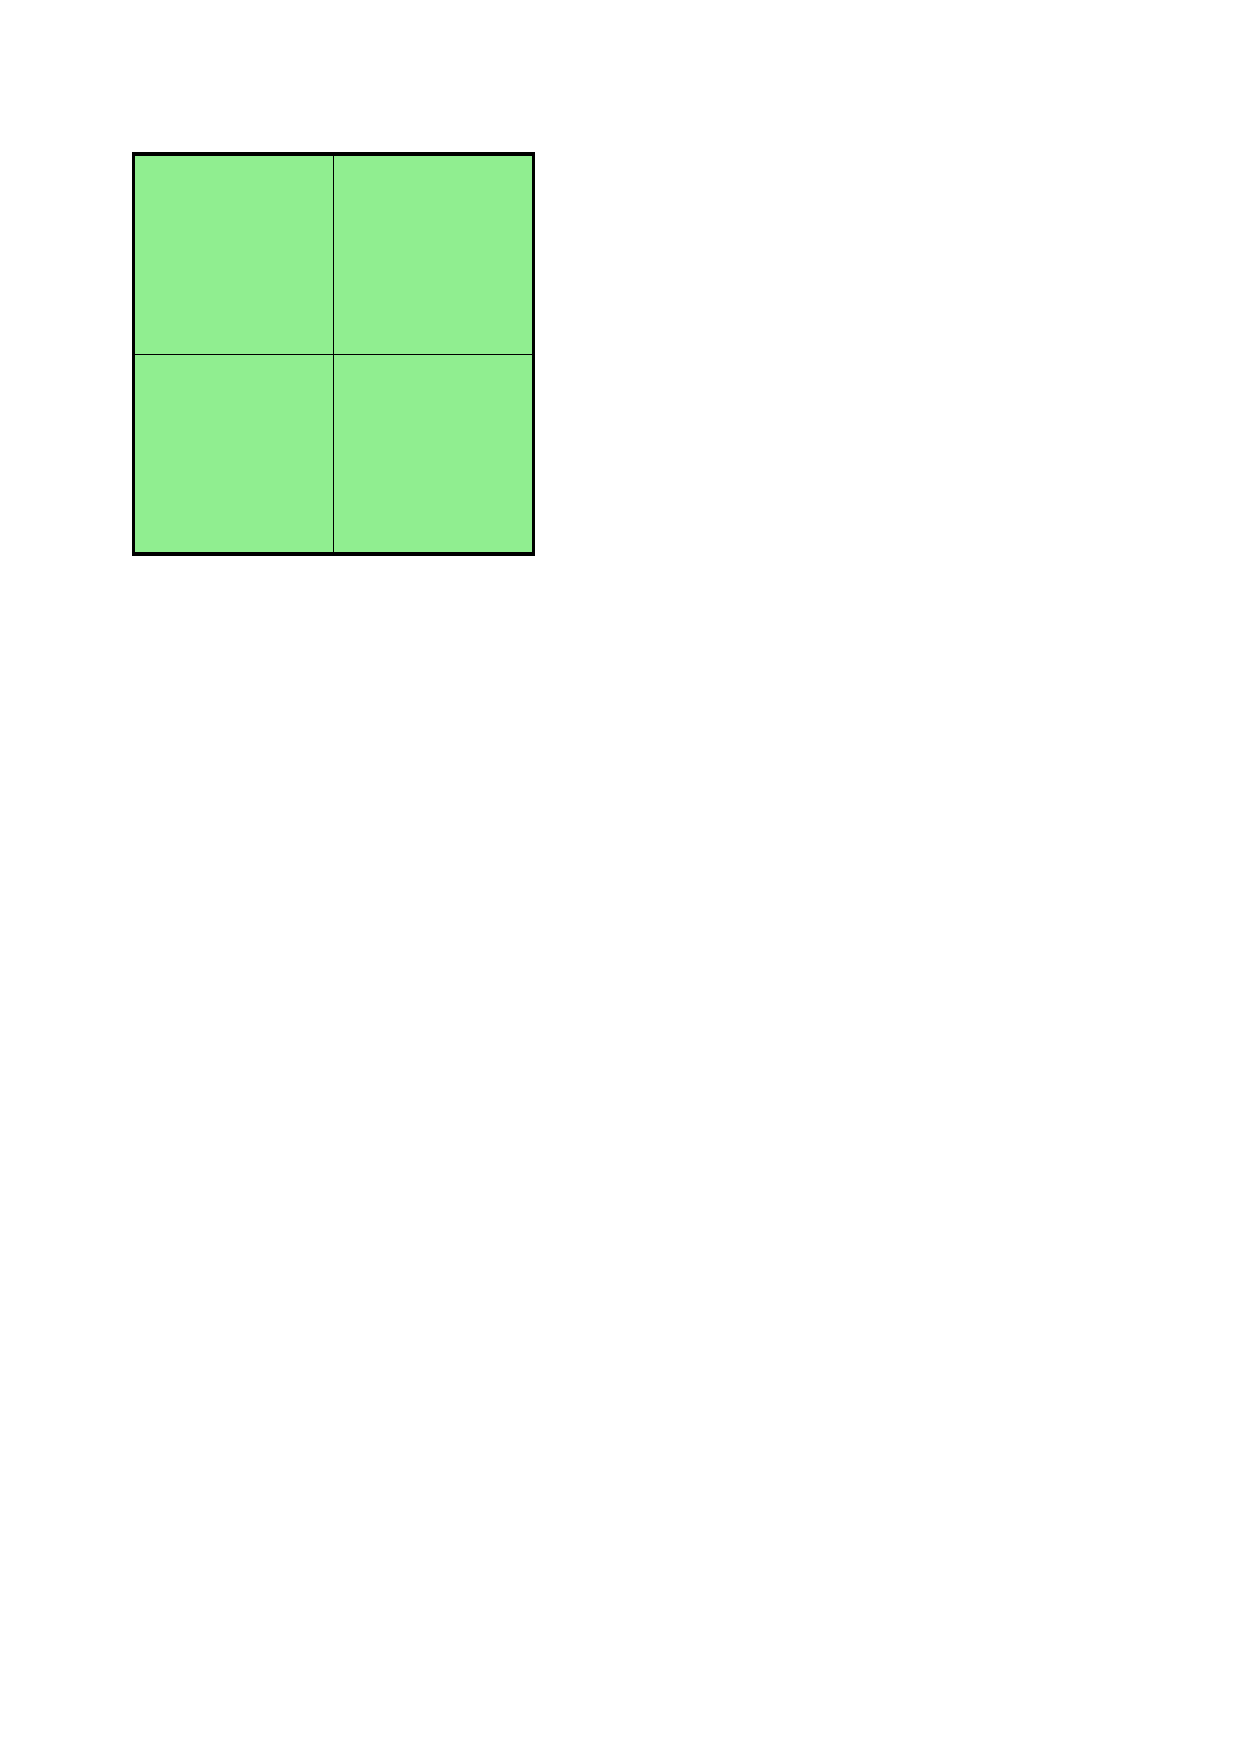
\includegraphics[scale=\normalipe]{ch01-ctverec-sobepodobnost.pdf}
        \caption{Čtverec rozdělený na čtyři menší čtverce.}
        \label{subfig:sobepodobnost-ctverce-1}
    \end{subfigure}
    \begin{subfigure}[b]{\subfigwidth}
        \centering
        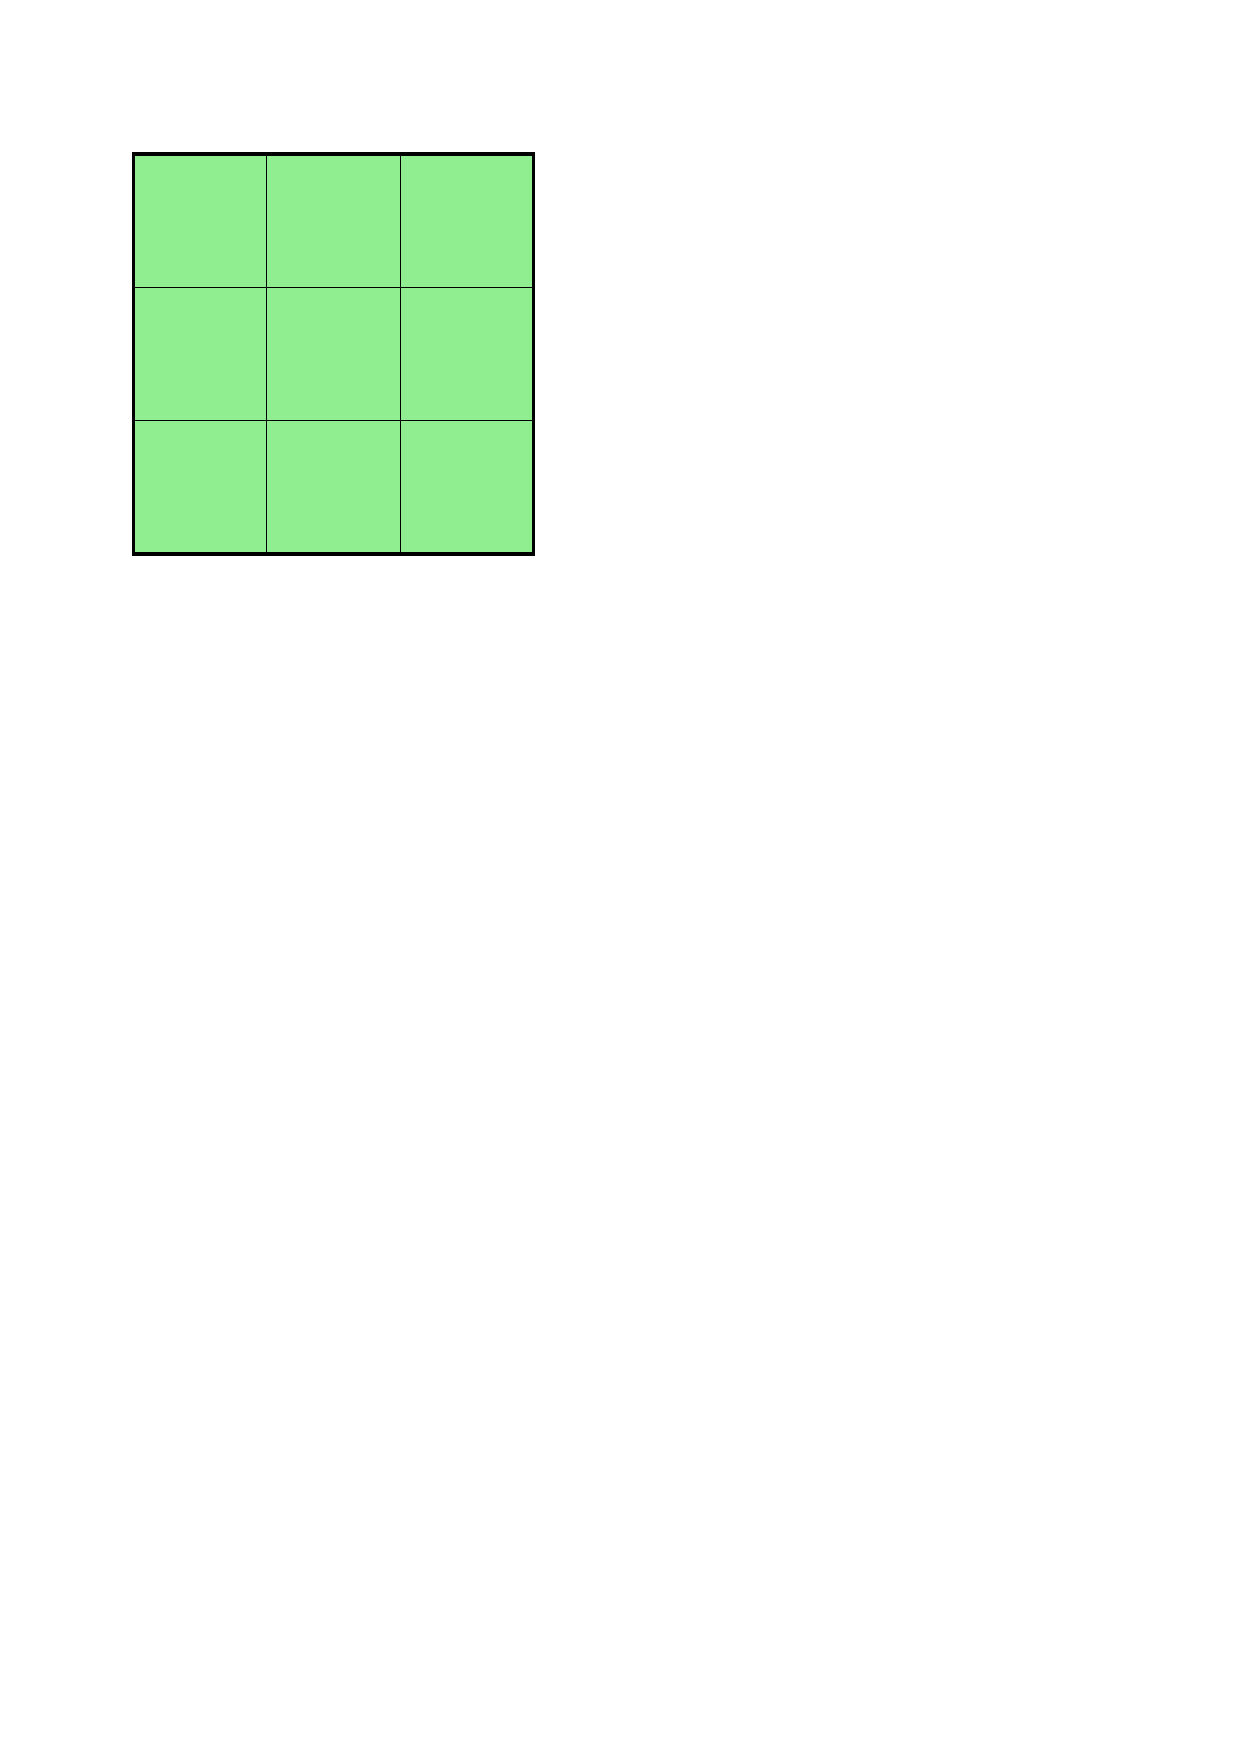
\includegraphics[scale=\normalipe]{ch01-ctverec-sobepodobnost-2.pdf}
        \caption{Jiná možnost rozdělení čtverce.}
        \label{subfig:sobepodobnost-ctverce-2}
    \end{subfigure}
    \caption{Soběpodobnost čtverce.}
    \label{fig:sobepodobnost-ctverce}
\end{figure}
Podobně např. i obyčejná úsečka je taktéž soběpodobná, protože ji můžeme rozdělit na obecně $k$ stejných částí (viz obrázek \ref*{fig:sobepodobnost-usecky}).\par
\begin{figure}[h]
    \centering
    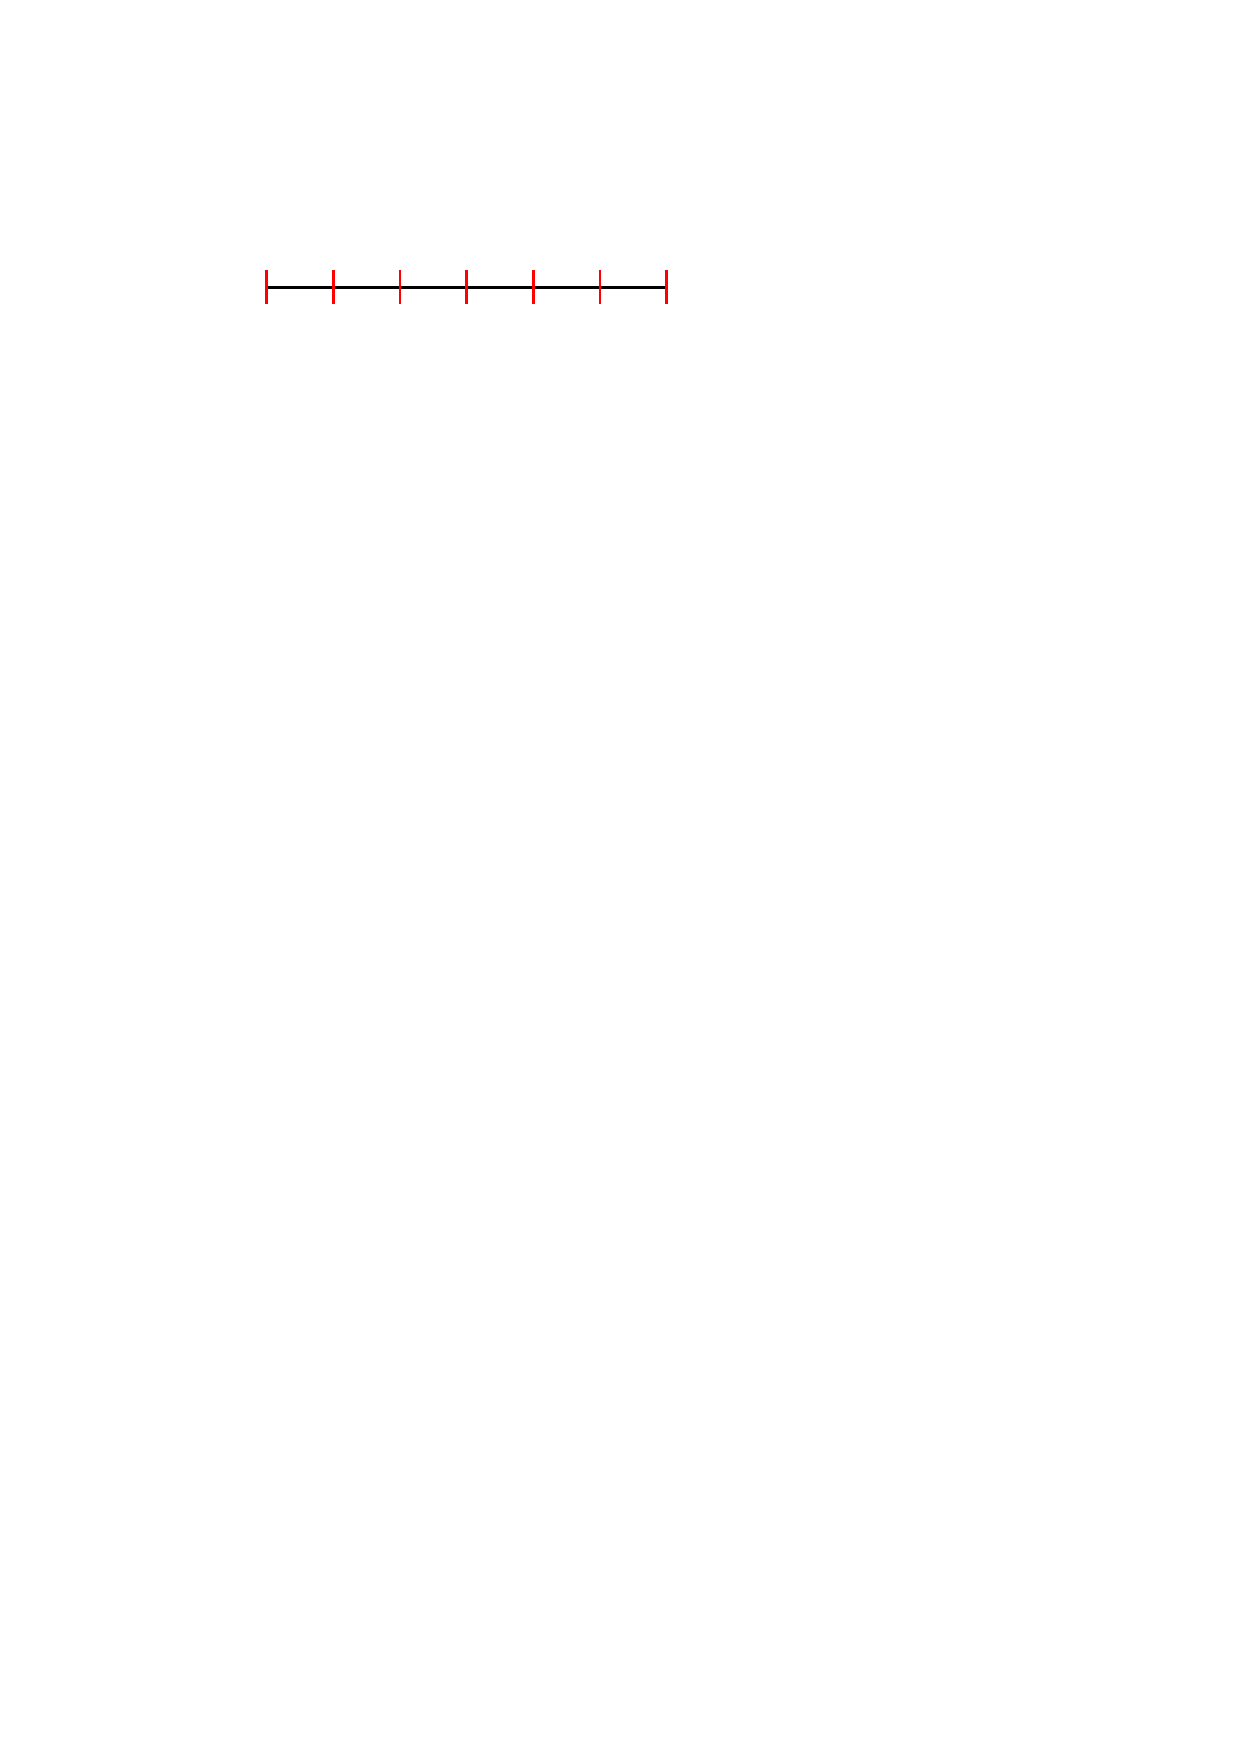
\includegraphics[scale=\normalipe]{ch01-usecka-sobepodobnost.pdf}
    \caption{Úsečka rozdělená na šest stejných částí.}
    \label{fig:sobepodobnost-usecky}
\end{figure}
K čemu nám takové uvědomnění vlastně je? Zmenšíme-li úsečku $k$-krát, pak budeme potřebovat přesně $k$ těchto částí, abychom dostali úsečku původní délky. U čtverce (nebo obdélkuníku obecně) při změnšení délky strany $k$-krát budeme potřebovat $k^2$ daných útvarů pro obdržení čtverce s původním obsahem.\footnote{Obdélník změnšený $k$-krát bude mít strany délek $a/k,\,b/k$, tedy jeho obsah bude
\[\dfrac{ab}{k^2}=\dfrac{S}{k^2},\]
kde $S$ je obsah původního obdélníka.}
Pro krychli bude situace zcela analogická, $k$-krát zmenšená kopie bude potřeba $k^3$-krát, abychom dostali krychli o původním objemu (viz obrázek \ref{fig:krychle-sobepodobnost}).
\begin{figure}[h]
    \centering
    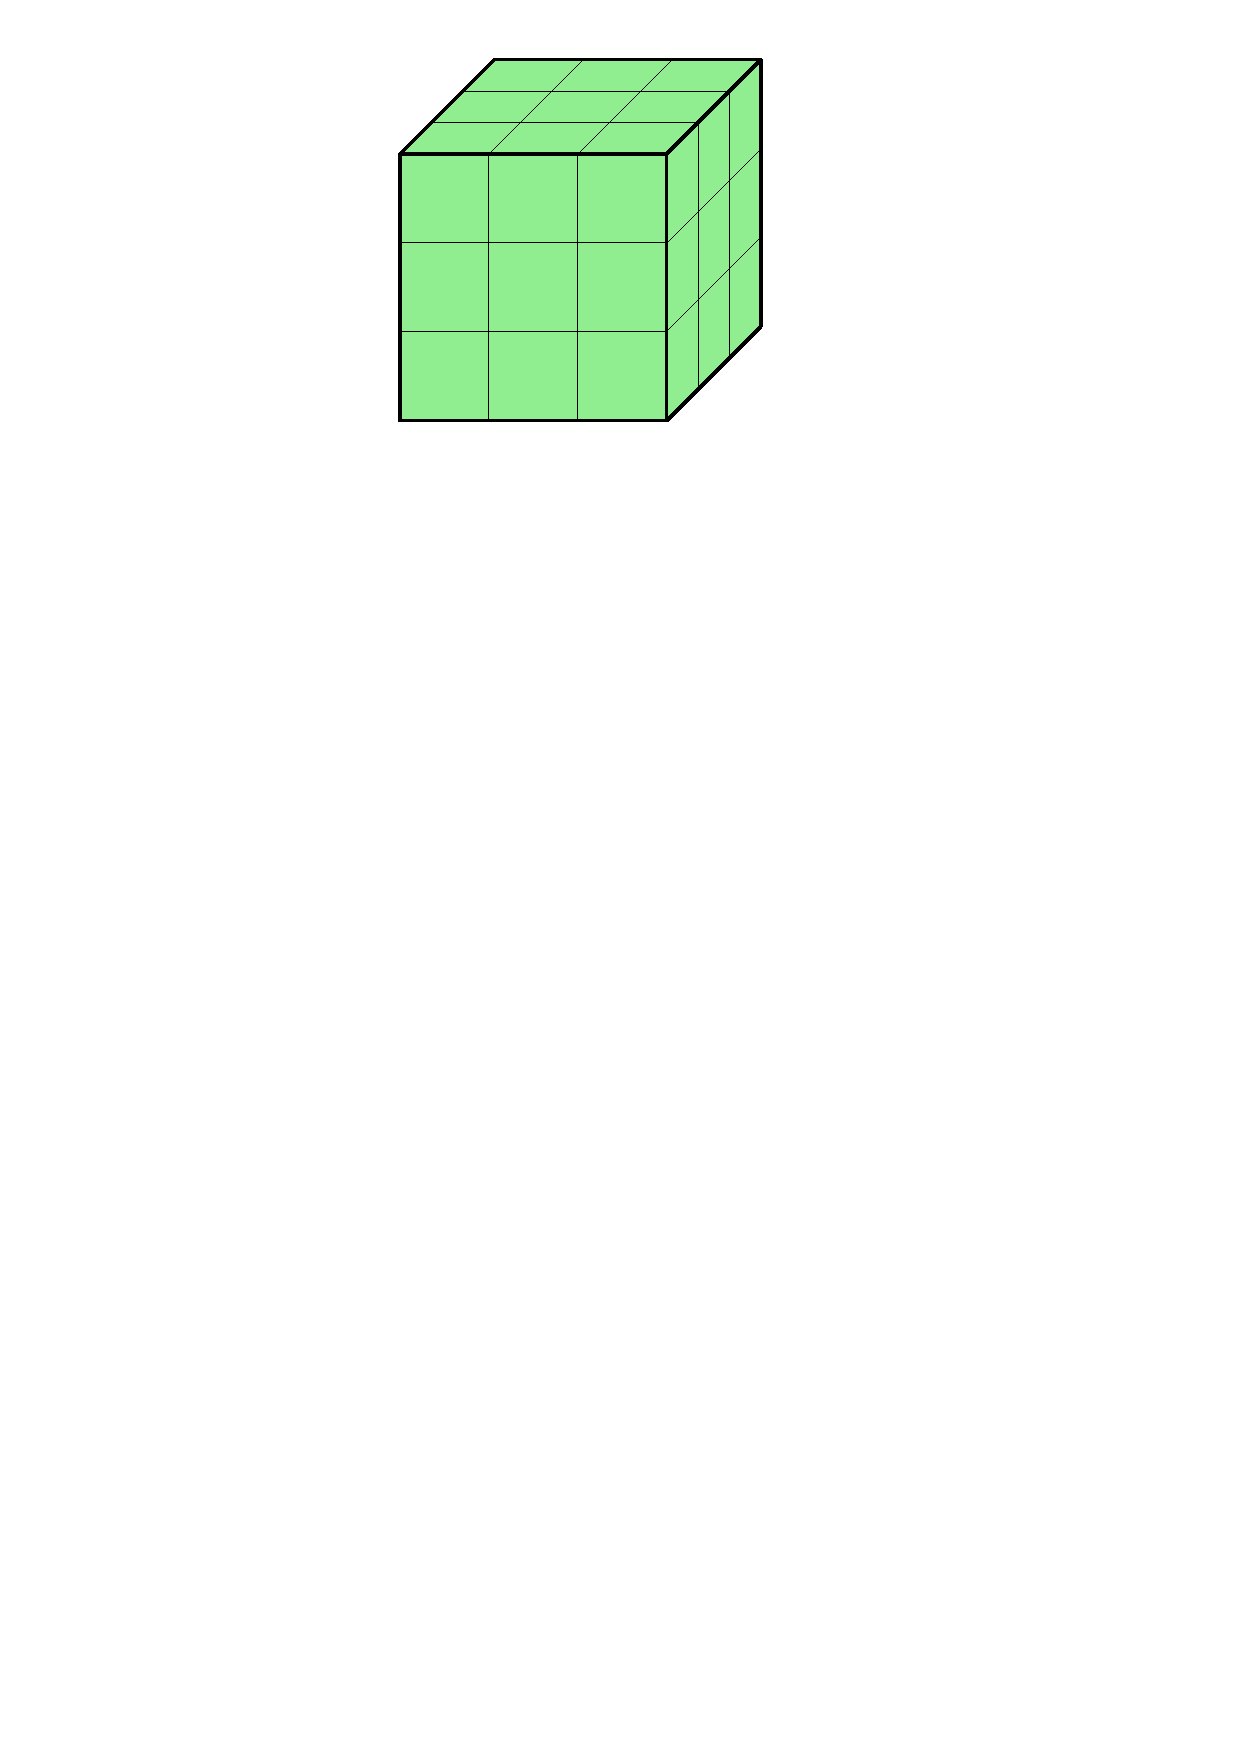
\includegraphics[scale=\normalipe]{ch01-krychle-sobepodobnost.pdf}
    \caption{Krychle rozdělená na 27 stejných částí.}
    \label{fig:krychle-sobepodobnost}
\end{figure}
Lze si všimnout, že v závislosti na \emph{dimenzi} objektu se mění daný exponent. Vztah lze tak zobecnit na
\begin{equation}\label{eq:pocet-utvaru}
    N(k)=k^d
\end{equation}
kde $N(k)$ je počet nových útvarů v závislosti na faktoru $k$ a $d$ je dimenze.\par
Toto je jeden z možných způsobů, jak lze chápat koncept dimenze. Jednoduchou úpravou rovnosti \eqref{eq:pocet-utvaru} dostaneme
\[d=\log_k{N(k)}=\dfrac{\ln{N(k)}}{\ln{k}}.\]
(Obecně lze volit jakýkoliv přípustný základ logaritmů, tj $d=\log_b{N(k)}/\log_b{k}$ pro $b\in\R^+\setminus\set{1}$.)
\begin{table}[h]
    \centering
    \begin{tabular}{r|cc}
    Útvar    & $N(k)$ & $d=\log_3{N(k)}/\log_3{k}$ \\ \hline
    Úsečka   & $3$      & $1$                          \\
    Čtverec  & $9$      & $2$                          \\
    Krychle  & $27$     & $3$                          \\
    Teserakt & $81$     & $4$                          \\
    \end{tabular}
    \caption{Hodnoty dimenze $d$ pro různé útvary.}
    \label{table:eukleides-dimenze}
\end{table}
Dimenze v tomto pojetí skutečně dává dobrý smysl. Pro "klasické" geometrické objekty vychází dimenze vždy celočíselně.\par
Na této myšlence je založen pojem tzv. \emph{fraktální dimenze}\footnote{Někdy se též nazývá \emph{Kolmogorovova dimenze} nebo \emph{Hausdoffova-Besikovičova dimenze}. Je pojmenována po německém matematikovi \name{Felixi Hausdorffovi} (1869--1942) a ruských matematicích \name{Andreji Kolmogorovovi} (1903--1987) a \name{Abramovi Besikovičovi} (1891--1970).}. Existuje více způsobů její definice. Jedna z nich, které se dále nyní v této sekci budeme držet, se v anglicky psané literatuře nazývá \emph{"box-counting dimension"}, odkud plyne i značení $\dimB$. Pro útvar $F$ (formálně vzato množinu bodů) definujeme 
\begin{equation}\label{eq:fraktalni-dimenze}
    \dimB{F}=\lim_{\varepsilon\to 0^+}{\dfrac{\ln{N_\varepsilon(F)}}{\ln{\left(\dfrac{1}{\varepsilon}\right)}}}.
\end{equation}
(Převzato z \cite[str. 93]{Zelinka2006} a \cite[str. 28]{Falconer2014}.) Výraz $1/\varepsilon$ zde představuje faktor podobnosti jako původní $k$ (samotné $\varepsilon$ tak hraje roli měřítka), avšak největší rozdíl zde představuje zkoumání "limitního chování" daného výrazu.
\begin{example}[Fraktální dimenze úsečky]\label{ex:fraktalni-dimenze-usecka}
    Začněme asi nejednodušším příkladem výpočtu fraktální dimenze, a to u úsečky (označme $\ell$). Představme si, že úsečku \emph{jednotkové délky} rozdělíme na $N_\varepsilon(\ell)=n$ shodných dílů. Pak měřítko libovolného dílu je
    \[\varepsilon=\dfrac{1}{n}=n^{-1}.\]
    (Zde je dobré si uvědomit, že pro $n\to\infty$, tedy zjemňování dělení úsečky, platí, že $\varepsilon\to 0^+$.) Fraktální dimenzi úsečky vypočteme z definice jako
    \[\dimB{\ell}=\lim_{\varepsilon\to 0^+}{\dfrac{\ln{N_\varepsilon(\ell)}}{\ln{\left(\dfrac{1}{\varepsilon}\right)}}}=\lim_{n\to\infty}{\dfrac{\ln{n}}{\ln{n}}}=1.\]
\end{example}
\begin{example}[Fraktální dimenze čtverce]\label{ex:fraktalni-dimenze-ctverec}
    Podobně, jako v příkladu \ref{ex:fraktalni-dimenze-usecka} výše, můžeme stanovit i fraktální dimenzi čtverce (označme $S$). Uvažujme tedy čtverec o jednotkovém obsahu, který rozdělíme $N_\varepsilon(S)=n$ shodných útvarů. Přitom víme, že obsah mění kvadraticky vůči délce strany. Měřítko nového čtverce tak bude
    \[\varepsilon=\sqrt{\dfrac{1}{n}}=n^{-1/2}\]
    a fraktální dimenze vychází
    \[\dimB{S}=\lim_{n\to\infty}{\dfrac{\ln{n}}{\ln{n^{1/2}}}}=\lim_{n\to\infty}{\dfrac{\ln{n}}{\dfrac{1}{2}\ln{n}}}=2.\]
\end{example}
Pro krychli bude výpočet naprosto analogický (viz příklad \ref{ex:fraktalni-dimenze-ctverec}). Obecně pro $d$-rozměrnou krychli bude její fraktální dimenze\footnote{Obdobnou úvahou dojmeme k měřítku $\varepsilon=n^{-1/d}$.} rovna $d$.\par
Zkusme se nyní odprostit od krychle k trochu jinému útvaru.
\begin{example}[Fraktální dimenze trojúhelníku]\label{ex:fraktalni-dimenze-trojuhelnik}
    Podívejme se, jak to dopadne s fraktální dimenzí \emph{obecného trojúhelníku}. Každý trojúhelník $T$ lze rozdělit na čtveřici \emph{vzájemně shodných trojúhelníků $T_1,\dots,T_4$}, které vzniknou sestrojením středních příček v původním trojúhelníku (viz obrázek \ref{fig:trojuhelnik-sobepodobnost}).
    \begin{figure}[h]
        \centering
        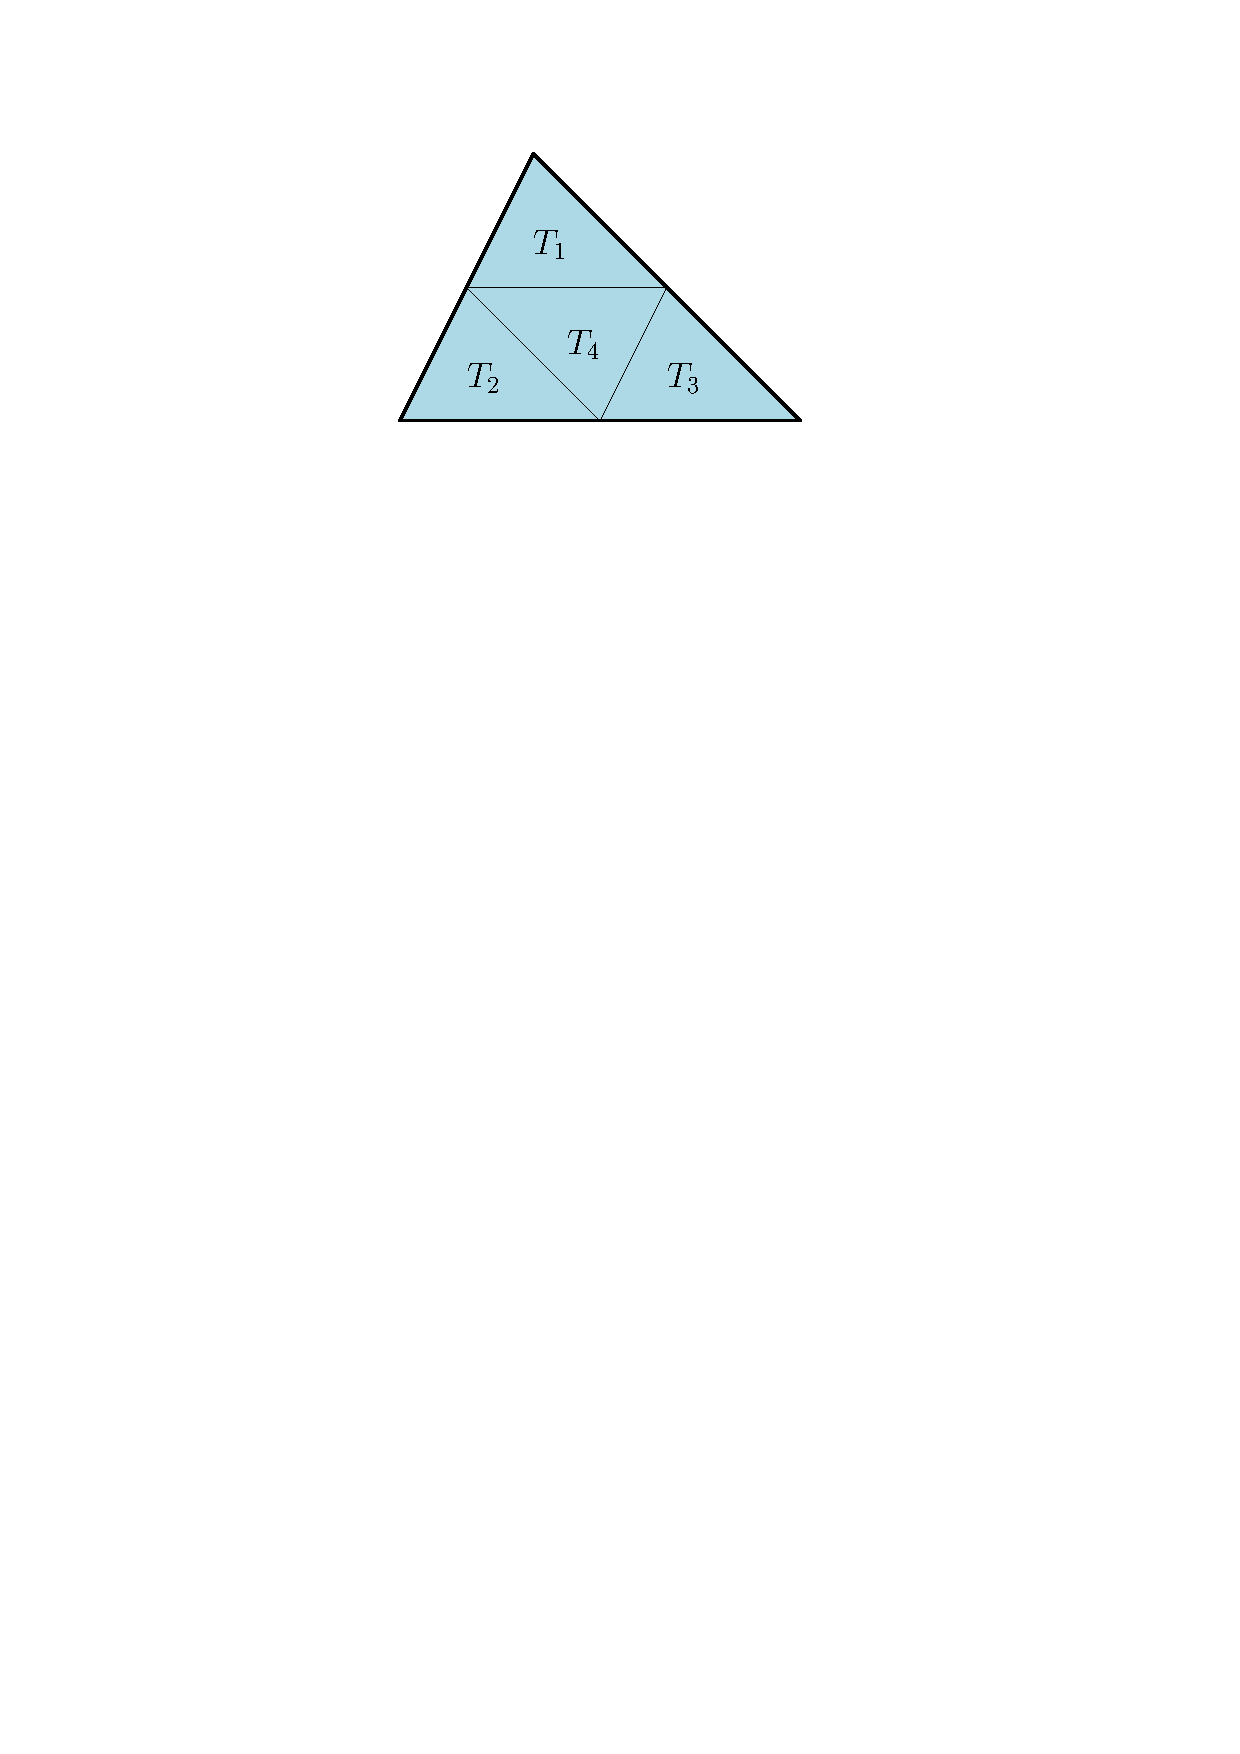
\includegraphics[scale=\normalipe]{ch01-trojuhelnik-sobepodobnost.pdf}
        \caption{Trojúhelník $T$ rozdělený na trojúhelníky $T_1,\dots,T_4$.}
        \label{fig:trojuhelnik-sobepodobnost}
    \end{figure}
    Délka každé střední příčky odpovídá polovině délky strany, s níž je rovnoběžná, tedy obsah každého z nich je \emph{čtvrtina obsahu původního} trojúhelníku $T$. Pokud obecně trojúhelník $T$ rozdělíme\footnote{Výpočet bychom mohli i zde provést ve stejném duchu jako u úsečky, čtverce nebo krychle. Počet částí, na než rozdělíme trojúhelník, označíme $N_\varepsilon(T)=n$, přičemž měřítko pak bude $\varepsilon=n^{-1/2}$.} takto na obecně $N_\varepsilon(T)=4^n$ pro nějaké $n\in\N$ shodných částí, pak měřítko každé z nich bude $\varepsilon=(1/2)^n$. Fraktální dimenze tak výchází:
    \[\dimB{T}=\lim_{n\to\infty}{\dfrac{\ln{4^n}}{\ln{2^n}}}=\lim_{n\to\infty}{\dfrac{2n\ln{2}}{n\ln{2}}}=2.\]
\end{example}
Pro jednoduché útvary vychází dimenze tak, jak bychom mohli očekávat. K zajímavějším výsledkům však dospějeme u fraktálů, na něž se blíže podíváme v následující podsekci \ref{subsec:dimenze-fraktalu}.

\subsection{Dimenze fraktálů}\label{subsec:dimenze-fraktalu}

Co kdybychom však zkusili podobnou myšlenku aplikovat i na \emph{fraktální objekty}? Zkusme to. Pro připomenutí jednotlivých křivek a výsledků k nim si dovoluji čtenáře opětovně odkázat na sekci \ref{sec:sobepodobnost}, kde jsou podrobněji rozebrány.
\begin{itemize}
    \item \textbf{Kochova křivka $F_{KC}$.} V každé iteraci nahrazujeme každou úsečku čtyřmi novými. Kompletní Kochova křivka tak obsahuje právě \emph{čtyři} kopie sebe sama zmenšených na třetinu, tj. v $n$-té iteraci je $N_\varepsilon(F_{KC})=4^n$, jak jsme již odvodili (viz podsekce \ref{subsec:kochova_krivka}).\footnote{Lze však zvolit i jiné dělení. Např. lze na Kochovu křivku nahlížet, že obsahuje \emph{16 kopií} sebe sama zmenšených na \emph{devítinu}.} Měřítko nové křivky je tak $\varepsilon=(1/3)^n$.
    \begin{equation}\label{eq:kochova-krivka-dimenze}
        \dimB{F_{KC}}=\lim_{\varepsilon\to 0^+}{\dfrac{\ln{N_\varepsilon(F_{KC})}}{\ln{\left(\dfrac{1}{\varepsilon}\right)}}}=\lim_{n\to\infty}{\dfrac{\ln{4^n}}{\ln{3^n}}}=\dfrac{\ln{4}}{\ln{3}}\approx 1{,}2618595\dots
    \end{equation}
    \item \textbf{Kochova vločka $F_{KS}$.} Začínáme s rovnostranným trojúhelníkem o straně délky $1$, na jehož stranách postupně vznikne Kochova křivka. V $n$-té iteraci je obvod Kochovy vločky $o_n$ roven $3\cdot 4^n$, tj. i $N_\varepsilon(F_{KS})=3\cdot 4^n$, kde měřítko\footnote{Měřítko se ve srovnání s Kochovou křivkou liší v mocnině, neboť délku nových úseků porovnáváme s obvodem celého trojúhelníku, nikoliv pouze délkou jedné jeho strany. Nicméně ve výpočtu bych se mohli omezit i jen na jednu ze stran, výpočet by byl tak zcela identický, jako u Kochovy křivky.} nově vzniklých úseček je $\varepsilon=1/3\cdot(1/3)^n=(1/3)^{n+1}$. Není těžké se přesvědčit, že fraktální dimenze vychází stejně, jako u Kochovy křivky:
    \begin{equation}\label{eq:kochova-vlocka-dimenze}
        \dimB{F_{KS}}=\lim_{n\to\infty}{\dfrac{\ln{3\cdot 4^n}}{\ln{3^{n+1}}}}=\lim_{n\to\infty}{\dfrac{\ln{4^n}\overbrace{\left(1+\dfrac{\ln{3}}{\ln{4^n}}\right)}^{\to 1}}{\ln{3^n}\underbrace{\left(1+\dfrac{\ln{3}}{\ln{3^n}}\right)}_{\to 1}}}=\dfrac{\ln{4}}{\ln{3}}
    \end{equation}
    \todo{Jak to bude s varinatou výpočtu pro plochu?}
    \item \textbf{Sierpińského trojúhelník $F_{ST}$.} V každé iteraci vynecháme prostřední trojúhelník, čímž vznikne \emph{trojice} nových trojúhelníků s \emph{polovičním} měřítkem. Tzn. $N_\varepsilon(F_{ST})=3^n$ pro $\varepsilon=(1/2)^n$, a tedy
    \begin{equation}\label{eq:sierpinskeho-trojuhelnik-dimenze}
        \dimB{F_{ST}}=\lim_{n\to\infty}{\dfrac{\ln{3^n}}{\ln{2^{n}}}}=\dfrac{\ln{3}}{\ln{2}}\approx 1{,}5849625\dots
    \end{equation}
    \item \textbf{Cantorovo diskontinuum $F_{CD}$.} Vždy vyjmeme prostřední třetinu úsečky, čímž obdržíme \emph{dvojici} úseček \emph{třetinové} délky, tj. $N_\varepsilon(F_{CD})=2^n$ pro $\varepsilon=(1/3)^n$. Fraktální dimenze tak vychází
    \begin{equation}\label{eq:cantorovo-diskontinuum-dimenze}
        \dimB{F_{CD}}=\lim_{n\to\infty}{\dfrac{\ln{2^n}}{\ln{3^n}}}=\dfrac{\ln{2}}{\ln{3}}\approx 0{,}6309297\dots
    \end{equation}
\end{itemize}
Udělejme si nyní menší souhrn a porovnání dosavadně získaných výsledků (viz tabulka \ref{table:fraktaly-eukleides-dimenze}).
\begin{table}[h]
    \centering
    \begin{tabular}{r|ccc}
        Útvar $F$                & $\varepsilon$ & $N_\varepsilon(F)$ & $\dimB{F}$         \\ \hline
        Úsečka                   & $n^{-1}$      & $n$                & 1                  \\
        Čtverec                  & $n^{-1/2}$    & $n$                & 2                  \\
        Krychle                  & $n^{-1/3}$    & $n$                & 3                  \\
        Teserakt                 & $n^{-1/4}$    & $n$                & 4                  \\
        $d$-rozměrná krychle     & $n^{-1/d}$    & $n$                & $d$                \\
        Obecný trojúhelník       & $(1/2)^n$     & $4^n$              & 2                  \\
        Kochova křivka           & $(1/3)^n$     & $4^n$              & $1{,}2618595\dots$ \\
        Kochova vločka           & $(1/3)^{n+1}$ & $3\cdot 4^n$       & $1{,}2618595\dots$ \\
        Sierpińského trojúhelník & $(1/2)^n$     & $3^n$              & $1{,}5849625\dots$ \\
        Cantorovo diskontinuum   & $(1/3)^n$     & $2^n$              & $0{,}6309297\dots$ \\
    \end{tabular}
    \caption{Porovnání fraktálních dimenzí $d_k$ různých objektů.}
    \label{table:fraktaly-eukleides-dimenze}
\end{table}
Můžeme si všimnout, že zatímco u "klasických" objektů vychází fraktální dimenze \emph{celočíselná}, u (zmíněných) fraktálů vychází \emph{neceločíselně}, ba dokonce i iracionálně.

\subsection{Topologická dimenze}\label{subsec:topologicka-dimenze}

Výsledky z předešlé části \ref{subsec:dimenze-fraktalu} se můžou zdát poněkud překvapující. Jak je vůbec možné, že dimenze nemusí vycházet nutně celočíselná? Ač se to možná zdá jako nesmyslný výsledek, je třeba si uvědomit, jak vlastně koncept dimenze chápeme. Na jednu stranu na ni lze nahlížet jako na mocninu "s níž se zvyšuje" obsah/objem tělesa. Naopak čtenář znalý lineární algebry si možná vzpomene, že v této matematické disciplíně se na dimenzi nahlíží jako na \emph{mohutnost libovolné báze daného vektorového (pod)prostoru}, která naopak vychází vždy pouze celočíselně, avšak nelze s ní dobře zachytit hlubší detail geometrie u objektů, jako jsou právě fraktály.

Tím se dostáváme ještě k jednomu typu dimenzí, a to tzv. \emph{topologické dimenze}. Ty totiž daleko více odpovídají našemu intuitivnímu chápání tohoto pojmu, neboť se vždy jedná o celé číslo, jak ho známe ze školní geometrie. Existuje více topologických dimenzí\footnote{Jiným příkladem takové dimenze je \emph{induktivní dimenze}.}, které si, co do definice, obecně nejsou ekvivalentní, ačkoliv ve většině standardních případů splývají. My se zde pro ilustraci podíváme na tzv. \emph{Lebesgueovu pokrývací dimenzi} (dále jen již "topologickou dimenzi") pojmenovanou po francouzském matematikovi \name{Henri Lebesgueovi} (1875--1941). Myšlenka definice je založena na pokrývání objektu (formálně vzato \emph{množiny bodů}) tzv. \emph{otevřenými množinami}.\footnote{Otevřená množina je zobecnění pojmu otevřeného intervalu reálných čísel. Neformálně řečeno je to taková množina $X$, kde pro každý její bod $x\in X$ patří do této množiny i nějaké $\varepsilon$-okolí tohoto bodu (patří do ní i body, které jsou "dostatečně blízko").} Formální definici si zde v rámci zachování jednoduchosti odpustíme, avšak pro hlubší matematický základ si dovolím čtenáře odkázat např. na knihu \cite{Engelking1989}.

Obecně množina $X$ má topologickou dimenzi $\dimL{X}=n$, pokud $n$ je nejmenší číslo, takové, že pro každé pokrytí otevřenými množinami\footnote{Formálněji to znamená, že $A_1,\dots,A_n$ jsou otevřené množiny, takové, že platí $X\subseteq\bigcup_{i=1}^n{A_i}$.} $\mathcal{U}$ existuje zjemnění\footnote{Zjemněním pokrytí $\mathcal{U}$ nazýváme takové (pod)pokrytí $\mathcal{U}^\prime$ množiny $X$, kde každá množina $A_i^\prime\in\mathcal{U}^\prime$ je \emph{podmnožinou} nějaké množiny $A_j$ původního pokrytí $\mathcal{U}$.} $\mathcal{U}^\prime$, v němž každý bod $x\in X$ leží v průniku nejvýše $n+1$ množin pokrytí $\mathcal{U}$.

% Obecně množina $X$ má topologickou dimenzi $\dimL{X}=n$, pokud danou množinu nelze pokrýt\footnote{Formálněji to znamená, že $A_1,\dots,A_n$ jsou otevřené množiny, takové, že platí $X\subseteq\bigcup_{i=1}^n{A_i}$.} lib. otevřenými množinami, tak, že pro každé zjemnění $\mathcal{U}$ tohoto pokrytí platí, že každý jeho bod $x$ je obsažen v průniku nejvýše $n+1$ množin $\mathcal{U}$.

Tuto ideu si zkusmíme přiblížit na příkladu topologické dimenze úsečky (viz obrázek \ref{fig:usecka-zjemneni}).
\begin{figure}[h]
    \centering
    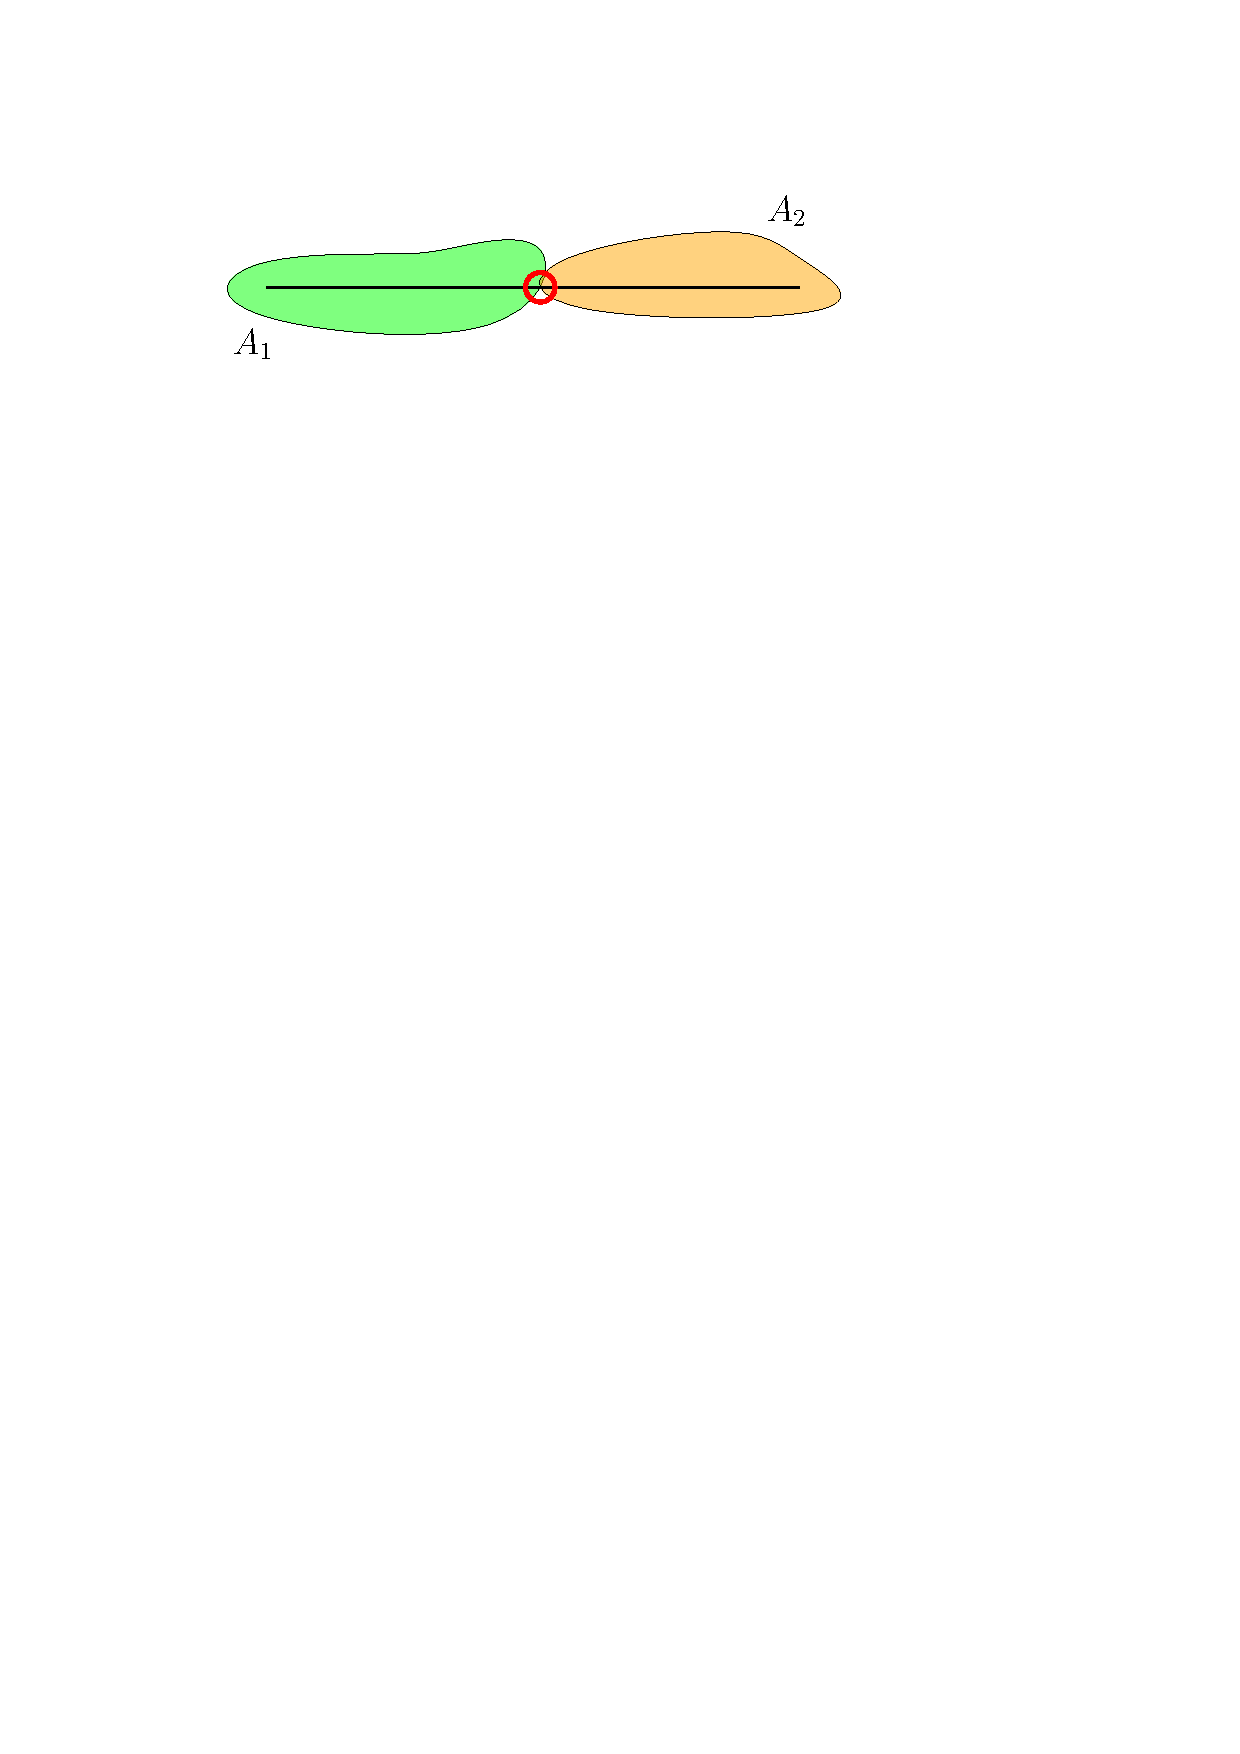
\includegraphics[scale=\normalipe]{ch01-usecka-pokryti-1.pdf}\\\qquad\\
    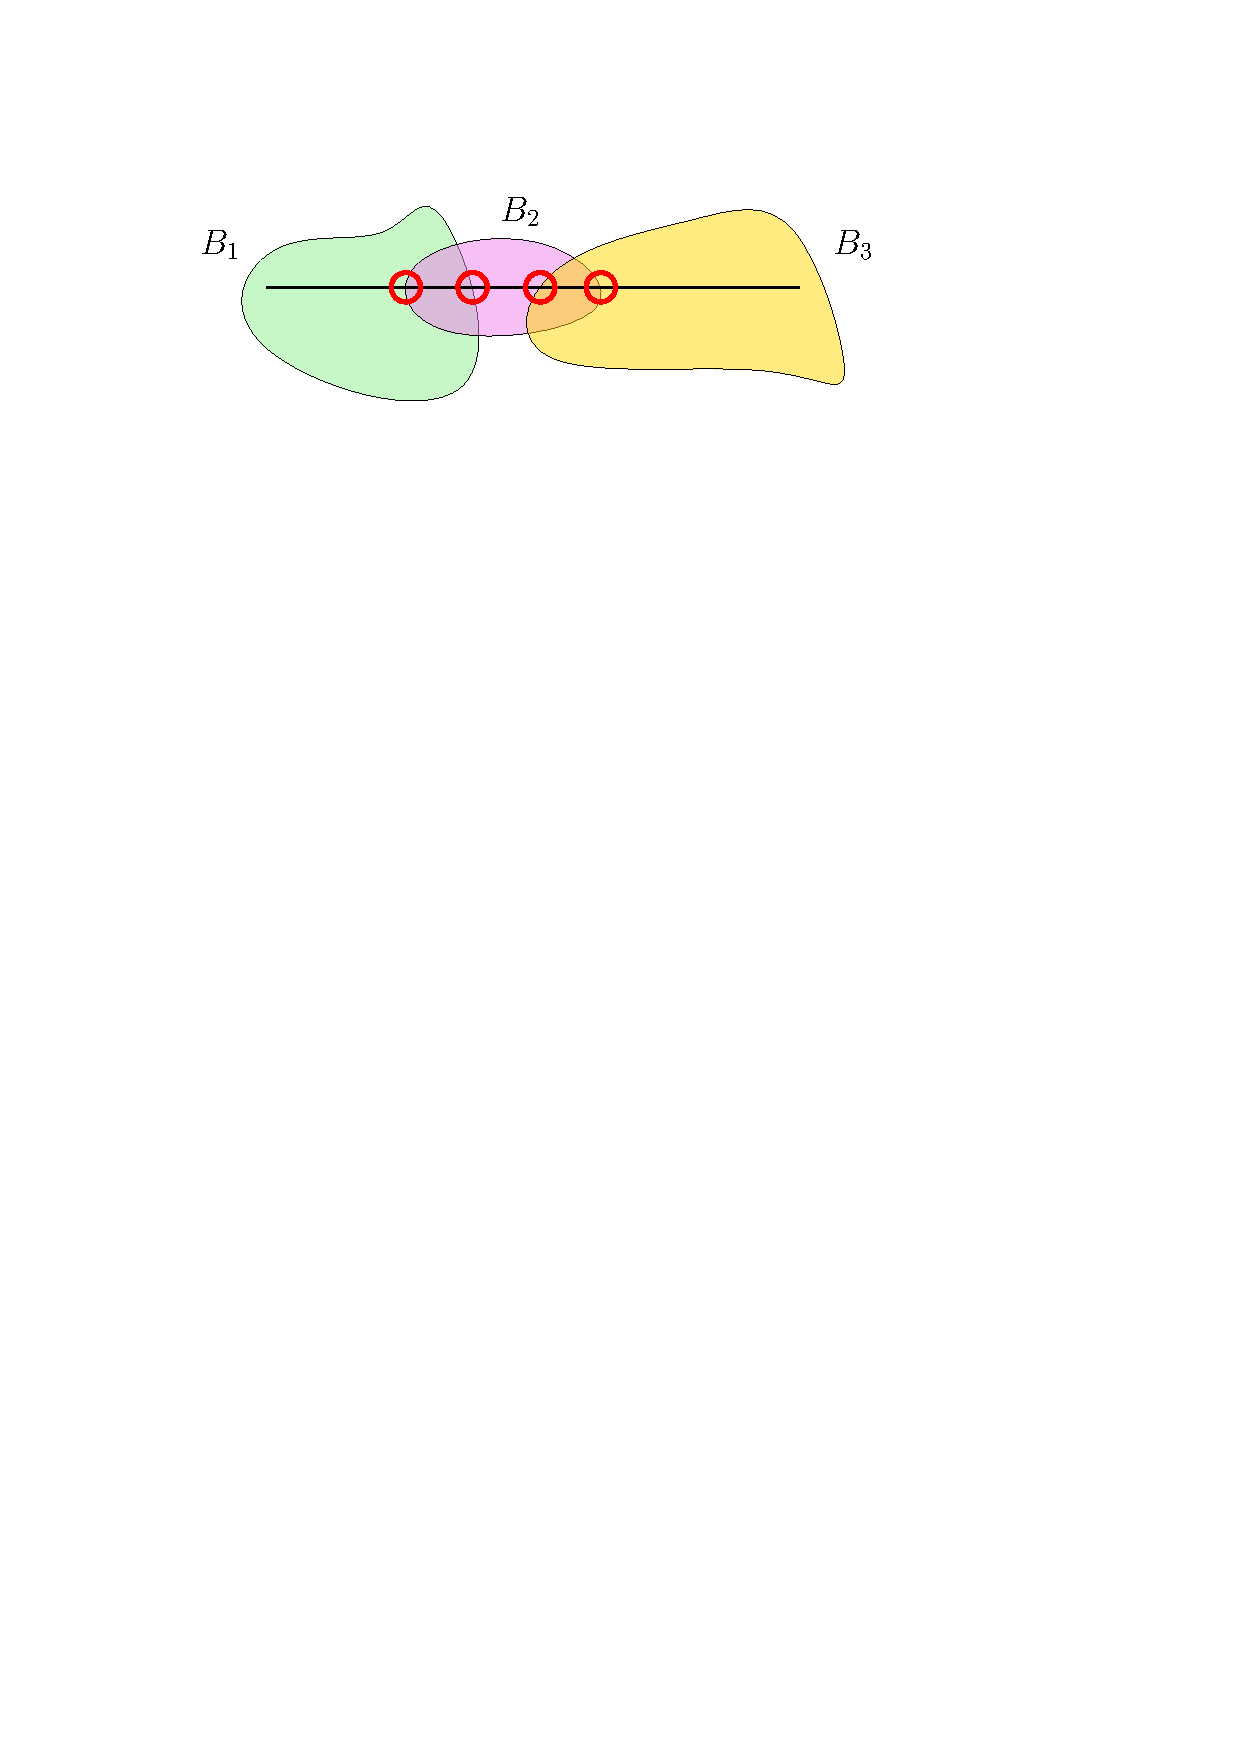
\includegraphics[scale=\normalipe]{ch01-usecka-pokryti-2.pdf}\\\qquad\\
    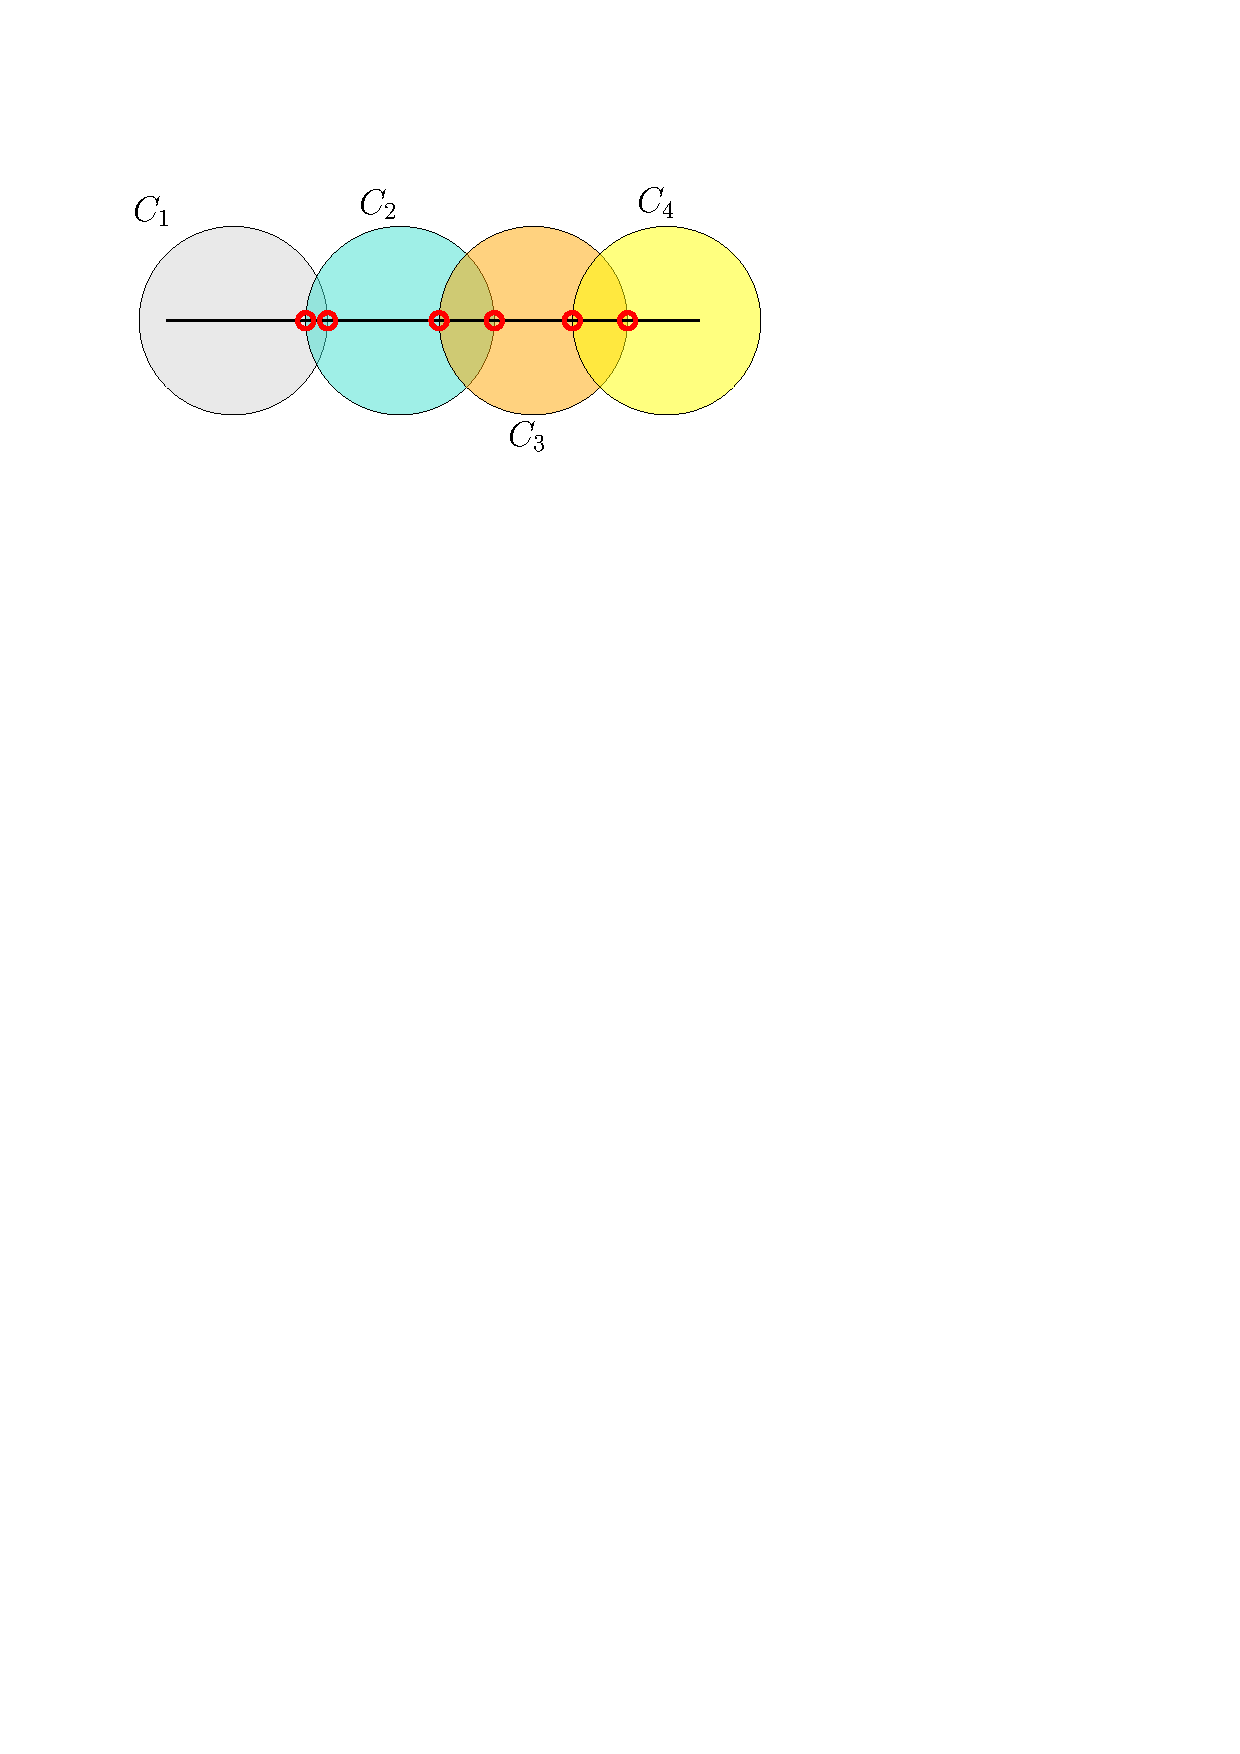
\includegraphics[scale=\normalipe]{ch01-usecka-pokryti-3.pdf}\\\qquad\\
    \caption{Různé možnosti (pod)pokrytí úsečky.}
    \label{fig:usecka-zjemneni}
\end{figure}
Pro libovolné pokrytí lze ukázat, že každý bod je obsažen v průniku maximálně \emph{dvou množin}, tedy topologická dimenze úsečky je $1$. Podobně např. pro čtverec lze dojít k závěru, že pro každé podpokrytí nějakého pokrytí je každý jeho bod obsažen v průniku maximálně \emph{tří množin}, tedy jeho topologická dimenze je 2, jak bychom očekávali (viz obrázek \ref{fig:ctverec-zjemneni}).
\begin{figure}[h]
    \centering
    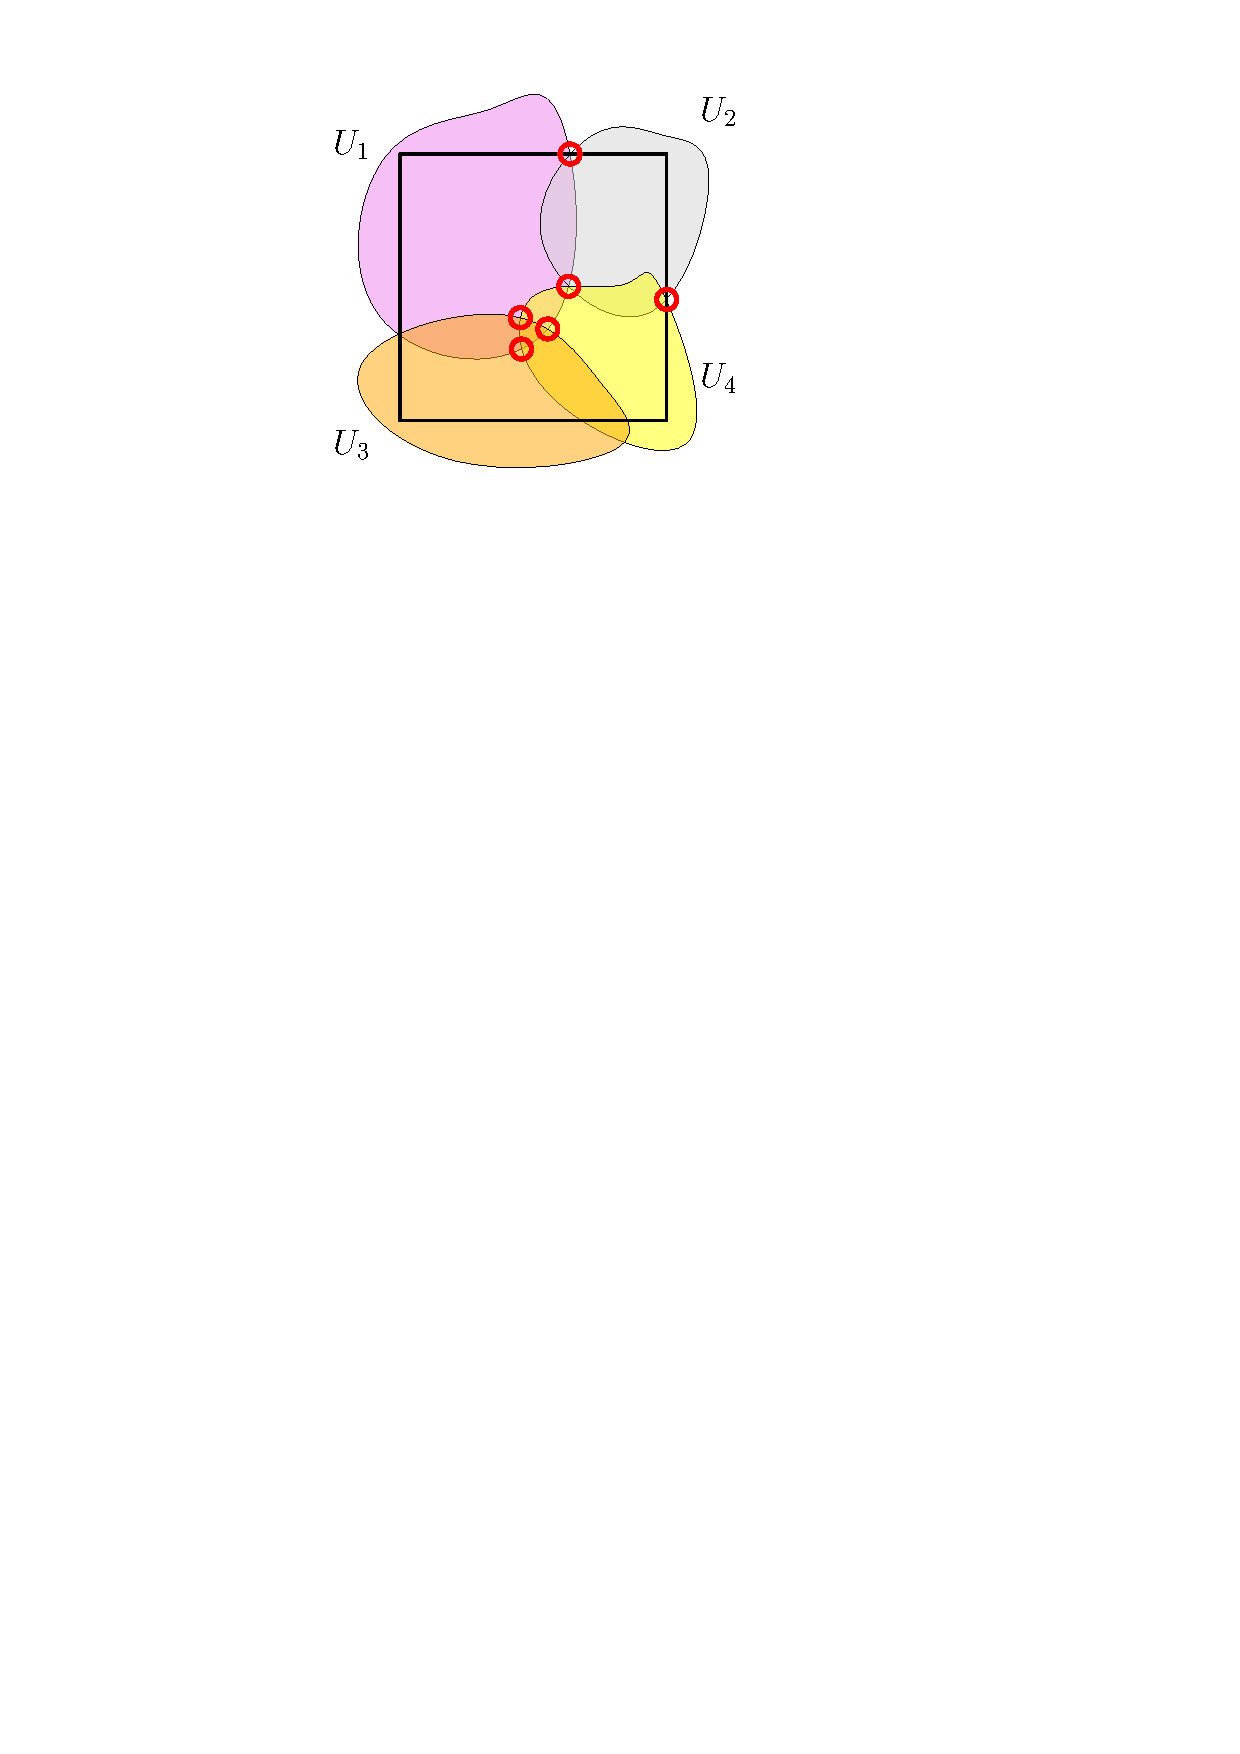
\includegraphics[scale=\normalipe]{ch01-ctverec-pokryti.pdf}
    \caption{Možné (pod)pokrytí čtverce.}
    \label{fig:ctverec-zjemneni}
\end{figure}
Jak jsme se již přesvědčili v příkladech \ref{ex:fraktalni-dimenze-usecka}, \ref{ex:fraktalni-dimenze-ctverec} a \ref{ex:fraktalni-dimenze-trojuhelnik}, pro "standardní" útvary je fraktální dimenze celočíselná (ač jsou i další, které jsme neuvedli), zatímco v podsekci \ref{subsec:dimenze-fraktalu} jsme zjistili, že u fraktální dimenze fraktálů tomu tak již nutně být nemusí. Přitom však topologická dimenze fraktálních útvarů je (a dokonce musí být) celočíselná (viz tabulka \ref{table:fraktalni-topologicka-dimenze}).
\begin{table}[h]
    \centering
    \begin{tabular}{r|cc}
    Útvar $F$                & $\dimB{F}$            & $\dimL{F}$ \\\hline
    Úsečka                   & 1                     & 1          \\
    Čtverec                  & 2                     & 2          \\
    Krychle                  & 3                     & 3          \\
    Teserakt                 & 4                     & 4          \\
    $d$-rozměrná krychle     & $d$                   & $d$        \\
    Kochova křivka           & $1{,}2618595\dots$    & 1          \\
    Kochova vločka           & $1{,}2618595\dots$    & 1          \\
    Sierpińského trojúhelník & $1{,}5849625\dots$    & 1          \\
    Cantorovo diskontinuum   & $0{,}6309297\dots$    & 0      
    \end{tabular}
    \caption{Porovnání fraktální a topologické dimenze útvarů.}
    \label{table:fraktalni-topologicka-dimenze}
\end{table}
Fraktální dimenze tak oproti té topologické daleko lépe zachycuje informaci o detailní geometrii daných objektů.